
\section{Principales Materiales Utilizados en Ingeniería Química}

Los materiales de construcción en ingeniería se clasifican por su composición atómica y estructura del material, pudiendose distinguir entre ellos, metálicos, cerámicos, polímeros y actualmente a esta categoría se le unen los materiales compuestos (\textit{composites}) y semiconductores.

\subsection{Metales y Aleaciones}
\textbf{Sustancias inorgánicas formadas por uno o mas elementos metálicos} (con posibles inclusiones de elementos no metalicos como C, N u O), con red cristalina ordenada y nube electrónica deslocalizada. Destacan por su excelente conductividad térmica y eléctrica, opacidad, superficie pulida y brillante, ductilidad a temperatura ambiente y alta resistencia mecánica (incluso a temperaturas elevadas en algunos casos). Son los materiales estructurales fundamentales de tuberías, columnas y recipientes a presión debido a que son resistentes y deformables.

\subsection{Materiales Cerámicos}
\textbf{Inorgánicos constituidos por elementos metálicos y no metálicos cohesionados químicamente} . Presentan altísima dureza, refractariedad (resistencia a temperaturas superiores a $1000^\circ\text{C}$), gran inercia química frente a ácidos concentrados, resistencia al desgaste y excelentes propiedades como aislantes térmicos y eléctricos. Sin embargo, su comportamiento es frágil (no presentan periodo de fluencia).
\begin{itemize}
    \item \textbf{Cerámicos tradicionales:} Arcillas, sílice ($\text{SiO}_2$) y feldespatos (empleados en ladrillos refractarios y revestimientos vitrificados) debido a que en ambientes químicos agresivos y temperaturas elevadas son mas resistentes que los metales y polímeros utilizandose de esta forma como aislantes y revestimiento de hornos (hornos cerámicos).
    \item \textbf{Cerámicos técnicos avanzados:} Alúmina ($\text{Al}_2\text{O}_3$) utilizado fundamentalmente como soporte de los circuitos integrados de los chips de ordenadores, carburo de silicio ($\text{CSi}$) y nitruro de silicio ($\text{Si}_3\text{N}_4$), utilizados en sellos mecánicos de bombas, álabes experimentales de turbinas y motores cerámicos debido a su resistencia a altas temperaturas y su bajo peso con lo que se consigue un mejor aprovechamiento del combustible y menor inercia de la maquina.
\end{itemize}
funciona muy mal con disoluciones basicas,los medios basicos atacan sobretodo a temperatura mayor los materiales ceramicos. se suelen usar cuando se necesita temperatura muy elevada con bajo peso en las turbinas de ingenieria
\subsection{Polímeros y Plásticos}
Compuestos orgánicos macromoleculares formados por \textbf{largas cadenas de moleculas orgánicas basadas en el carbono}. Se caracterizan por su baja densidad, alta flexibilidad, buen aislamiento eléctrico y resistencia a la corrosión acuosa, aunque presentan bajas temperaturas máximas de trabajo ($<150 - 250^\circ\text{C}$) y susceptibilidad a la termofluencia (ablandamiento a temperaturas bajas).
\begin{itemize}
    \item \textbf{Termoplásticos:} Cadenas lineales o ramificadas unidas por fuerzas débiles de Van der Waals. Pueden \textbf{ablandarse y deformarse por calor y moldearse repetidas veces} (polietileno PET/PE, cloruro de polivinilo PVC, polipropileno PP, poliestireno PS, PTFE teflón).
    \item \textbf{Termoestables:} Redes poliméricas tridimensionales altamente reticuladas mediante enlaces covalentes. \textbf{Al calentarse no se funden sino que se descomponen térmicamente}. Presentan \textbf{mayor rigidez, estabilidad dimensional y resistencia térmica que los termoplásticos, menor peso, mayor resistencia a la termofluencia y deformación bajo carga ademas de altas propiedades de aislamiento térmico y eléctrico} (resinas epoxídicas, poliésteres insaturados, resinas fenólicas).
\end{itemize}

\begin{table}[H]
    \centering
    \begin{tabular}{lcccc}
        \toprule
        \textbf{Material para tuberías}     & \textbf{$E$ ($10^5\text{ psi}$)} & \textbf{Resiliencia}                            & \textbf{$\sigma_M$ ($\text{psi}$)} & \textbf{$T_{\text{máx}}$ ($^\circ\text{F}$)} \\
        \midrule
        Polietileno (PE)                    & $0.2 - 0.6$                      & $>15\text{ ft}\cdot\text{lb}/\text{in}^2$       & $1400 - 2500$                      & 120                                          \\
        Policloruro de vinilo (PVC)         & $4.0 - 5.4$                      & $0.6 - 0.9\text{ ft}\cdot\text{lb}/\text{in}^2$ & $6400 - 9000$                      & 150                                          \\
        Epoxi reforzado con fibra de vidrio & 50                               & $>10\text{ ft}\cdot\text{lb}/\text{in}^2$       & $25000 - 30000$                    & 300                                          \\
        Acero al carbono                    & 300                              & Excelente                                       & 48000                              & 1000                                         \\
        Acero inoxidable austenítico        & 280                              & Excelente                                       & 75000                              & 1500                                         \\
        Cobre comercial                     & 70                               & Excelente                                       & 30000                              & 400                                          \\
        \bottomrule
    \end{tabular}
    \caption{Comparativa de propiedades de materiales habituales para conducciones y tuberías de proceso.}
    \label{tab:comparativa_tuberias}
\end{table}
lo que se suele buscar en los polimeros es que sean buenos aislantes, que sean flexibles sobretodo los termoplasticos, baja densidad pero tienen algunos incovenientes tiene temperatura de fluencia muy baja. Para resistencia mecanica mas elevada necesitamos ir a los termoestables y aun asi no todos sirven.
\subsection{Materiales Compuestos (\textit{Composites})}
Materiales multifásicos (\textbf{mezclas de dos o más materiales}) \textbf{formados por la combinación sinérgica de un material de refuerzo (fibras resistentes y rígidas) integrado en un aglomerante continuo o matriz} con una densidad relativamente baja (polimérica, metálica o cerámica).

La formación de un material compuesto se realiza distribuyendo un \textbf{material de relleno en una matriz, de forma que el relleno refuerce la matriz. El resultado es un material compuesto que tiene alta resistencia y rigidez en relación con su bajo peso.}
\begin{itemize}
    \item \textbf{Fibras de refuerzo:} Fibras de vidrio (Tipo E para uso general dieléctrico, Tipo S de alta resistencia mecánica), fibras de carbono (derivadas de poliacrilonitrilo PAN carbonizadas y grafitizadas a alta temperatura), y fibras de aramida aromática (\textbf{Kevlar}) de altísima absorción de impacto.
    \item \textbf{Propiedades específicas:} Presentan altísima resistencia específica ($\sigma_M/\rho$) y rigidez específica ($E/\rho$), superando ampliamente a los metales convencionales (acero, aluminio y titanio) con un peso muy inferior.
    \item \textbf{Limitaciones actuales:} Elevado coste de materias primas, anisotropía direccional de sus propiedades, técnicas de moldeo más complejas y límite térmico impuesto por la matriz polimérica ($<260^\circ\text{C}$).
\end{itemize}

\nt{Ejemplos característicos de los constituyentes de estos materiales son \textbf{la fibra de vidrio, las fibras de carbono y las fibras de aramidas en una matriz epoxídica}. Otro ejemplo es el sulfuro de polifenilo reforzado con fibra de vidrio que se utiliza en instalaciones de tuberías de campos petrolíferos y ofrece una alta resistencia a la corrosión.}
\nt{Otro ejemplo son las fibras de kevlar($\text{aramidas}$), debido a su alta resistencia y bajo peso se utiliza en la industria aeroespacial, chalecos antibalas y ropa de moto}

los materiales compuestos se usan cuando necesitas buena resistencia mecanica pero poco peso por ejemplo para uso aeronautico
\begin{figure}
    \centering
    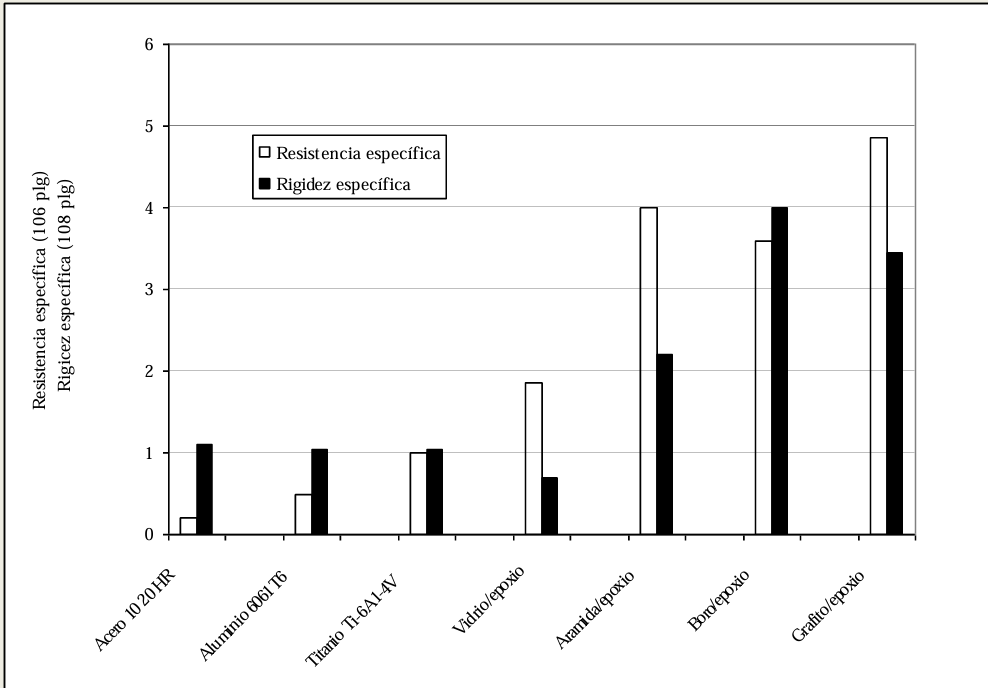
\includegraphics[width=0.4\textwidth]{kevlar.png}
    \caption{Comparativa de resistencia específica y rigidez específica de materiales compuestos y metalicos \\Fuente: diapositivas de la asignatura}
    \label{fig:comparativa_resistencia_rigidez}
\end{figure}

Como puede observarse los primeros muestran mayor resistencia con un menor peso.

\dfn{resistencia especifica}{Resistencia a la traccion dividida por la densidad \\ $\frac{\sigma}{\rho}$}
\dfn{rigidez especifica}{Modulo de Young(elasticidad) dividida por la densidad \\ $\frac{E}{\rho}$}

existen dos tipos de fibra de vidrio, el vidrio E y el vidrio E, La fibra de carbono se obtiene a partir del compuesto orgánico poliacrilonitrilo, mediante el proceso siguiente:
\begin{figure}
    \centering
    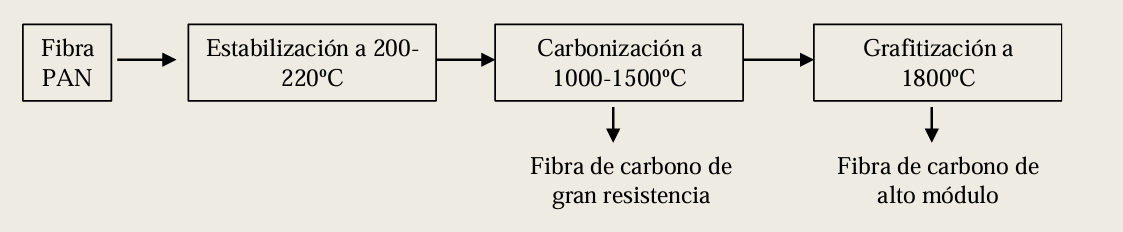
\includegraphics[width=0.4\textwidth]{fibra_de_vidrio.png}
    \caption{Proceso de obtencion de la fibra de vidrio}
    \label{fig:fibra_de_vidrio}
\end{figure}

En primer lugar son estirados y oxidados a temperaturas de 200-220ºC y, tras un proceso de carbonización que elimina O, H y N se produce la grafitización, donde el material sometido a altas temperaturas aumenta el grado de orientación de los cristales tipo grafito dentro de cada fibra.

\nt{Las propiedades mecánicas de los materiales compuestos dependen de su composición siendo asi, intermedias entre las propiedades mecánicas de las fibras y la matriz que forman el material compuesto.}

Por lo general las fibras presentan tensiones de resistencia máxima, límite de proporcionalidad, etc. mucho mayores que las de la matriz que forma el material, presentando el material compuesto un valor intermedio.

\begin{figure}
    \centering
    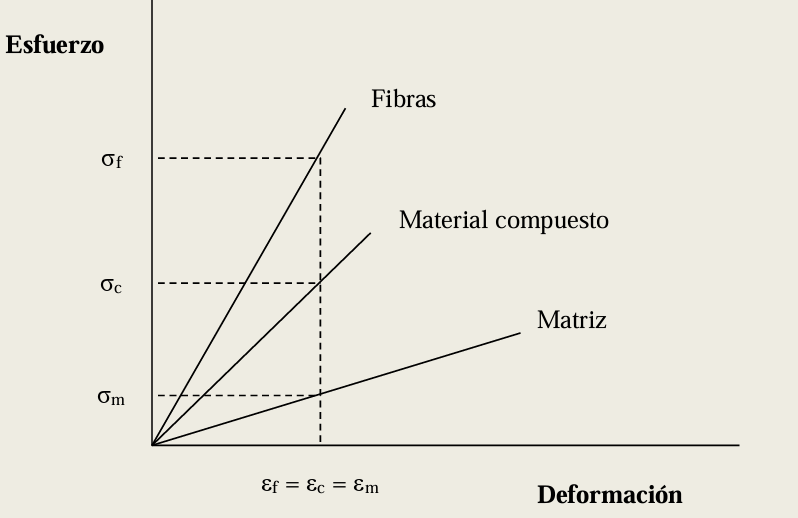
\includegraphics[width=0.4\textwidth]{fibras_vidrio_diagrama_esfuerzo_deformacion.png}
    \caption{Curvas tension-deformacion de materiales compuestos, fibras y matriz \\ Fuente: diapositivas de la asignatura}
    \label{fig:curvas_tension_deformacion}
\end{figure}
Las caracteristicas mas importantes son:
\begin{itemize}
    \item  La \textbf{resistencia máxima a la tracción específica} puede variar hasta cinco veces respecto a las aleaciones de alta resistencia. Los módulos de elasticidad específicos hasta ocho veces.
    \item  Los materiales compuestos pueden funcionar mucho mejor que el acero en aplicaciones donde existen \textbf{cargas cíclicas que produzcan fatiga}.
    \item  Donde se esperen \textbf{cargas de impacto y vibraciones} los materiales compuestos pueden proporcionar un alto nivel de amortiguación.
    \item Como las \textbf{propiedades} de estos materiales \textbf{cambian con la dirección} en las que se colocan las fibras, no son isotropicos, la fabricación de estos materiales se realiza procurando la máxima homogeneidad del material consiguiendo una distribución adecuada de las fibras en el interior del material.
    \item Los \textbf{cambios dimensionales con la temperatura suelen ser menores} en los materiales compuestos que en los metales.
    \item Pueden fabricarse \textbf{estructuras de formas complejas de una sola pieza} lo que reduce el número de operaciones de sujeción, se eliminan las juntas, etc.
\end{itemize}

Aunque estos materiales tienen una serie de \textbf{limitaciones} como son:
\begin{itemize}
    \item \textbf{El coste elevado de las materias primas} de la que están formados.
    \item Su fabricación requiere de \textbf{técnicas más complejas} que las de los materiales convencionales por lo que son distintas y poco generalizadas.
    \item Las \textbf{temperaturas máximas} que pueden soportar los materiales compuestos de matriz polimérica son 260ºC aunque esto puede modificarse con matrices cerámicas o metálicas.
    \item \textbf{Pueden presentar problemas de anisotropía direccional} de sus propiedades \textbf{es decir} que al \textbf{no} ser \textbf{isotrópicas varían con la dirección en la que se aplique la carga}.
    \item El análisis del comportamiento e inspección de estos materiales \textbf{requiere técnicas especiales} que aún no están totalmente desarrolladas.
\end{itemize}
la relacion resistencia coste que hay suele ser mayor en este tipo de materiales.

\subsection{Materiales Semiconductores}
Materiales con \textbf{propiedades de conductividad eléctrica intermedias entre conductores y aislantes fuertemente modulables por dopaje con impurezas atómicas, temperatura o campo eléctrico} (silicio monocristalino, germanio, arseniuro de galio GaAs). Constituyen la base de la instrumentación electrónica, en los \textbf{circuitos integrados} para la industria electrónica y ordenadores. El mas importante de estos es el \textbf{Silicio} puro,
que puede ser modificado para cambiar sus propiedades eléctricas, ya que éstas son extremadamente sensibles a la presencia de átomos de impurezas. También, el germanio, selenio, arseniuro de galio, seleniuro de cinc o teluro de plomo.

\subsection{Tendencia en el uso de materiales y criterios de selección}
los plásticos termoestables pueden utilizarse a temperaturas más altas que los materiales termoplásticos si bien se observa que la temperatura máxima de operación de los distintos materiales termoestables compuestos de matriz polimérica es baja, no superando los 300ºC. Los materiales metálicos son más adecuados cuando se necesitan materiales más resistentes por lo que son los más utilizados en la industria química como componentes fundamentales de las instalaciones.
\section{Aceros, Clasificación y Tratamientos}
\subsection{Sistemas de Clasificación y Nomenclatura (AISI / SAE y UNS)}
Existen organismos internacionales que regulan la nomenclatura de los metales:
\begin{itemize}
    \item \textbf{AISI / SAE:} Clasifica los aceros al carbono y aleados con un código de \textbf{4 dígitos}:
          \begin{itemize}
              \item Los dos primeros dígitos indican los elementos principales de aleación (ej. $10\text{xx}$ para acero al carbono ordinario, $11\text{xx}$ azufre de fácil mecanizado, $41\text{xx}$ cromo-molibdeno, $43\text{xx}$ níquel-cromo-molibdeno).
              \item Los dos últimos dígitos indican el contenido nominal medio de carbono expresado en centésimas de porcentaje (ej. el acero AISI 1020 posee un $0.20\%$ de C; el AISI 1045 un $0.45\%$ de C).
          \end{itemize}
    \item \textbf{Sistema de Numeración Unificada (UNS o SNU):} Código alfanumérico estandarizado por ASTM y SAE compuesto por una letra prefijo y cinco dígitos. Para aceros al carbono se emplea el prefijo \textbf{G} (ej. el AISI 1020 corresponde a UNS G10200). Para aceros inoxidables se emplea el prefijo \textbf{S} (ej. AISI 304 corresponde a UNS S30400).
\end{itemize}
las clasificaciones mas tipicas son la aisi, aa para el aluminio y ASTM
\subsection{Diagrama de Equilibrio Hierro-Carbono (Fe-C)}
Las aleaciones férreas se dividen en función de su porcentaje en masa de carbono:
\begin{itemize}
    \item \textbf{Aceros:} Contenido en carbono inferior al $1.76\%$ (o $2.14\%$ en clasificaciones termodinámicas clásicas).
    \item \textbf{Fundiciones:} Contenido en carbono entre el $2.14\%$ y el $6.67\%$ (límite correspondiente a la formación de cementita pura, $\text{Fe}_3\text{C}$).
\end{itemize}
\nt{lo que quiere es que sepamos que en los aceros de mas de un 6.67\% en carbono no se suele fabricar realmente es mucho mas abajo por que por debajo hay carburo de hierro, en los aceros se considera una aleacion de hierro con carburo de hierro,los que se suelen usar en ingenieria suelen ser de menor de 1.76\% se puede usar de mayor porcentaje que son fundiciones grises por ejemplo para bancos pero al ser demasiado rigidos no son tan utiles en la ingenieria
    para aceros con bajo porcentaje en carbono es ferrita mas carburo de hierro y a mas temperatura ?? si hacemos cambios de temperatura para tratamientos posteriores reducimos las tensiones superficiales pero no cambia la naturaleza}
\subsubsection{Fases y Constituyentes Microestructurales}
\begin{itemize}
    \item \textbf{Ferrita ($\alpha$):} Solución sólida intersticial de carbono en hierro BCC. Es la fase más blanda, dúctil y tenaz del acero (máxima solubilidad de carbono de $0.022\%$ a $727^\circ\text{C}$).
    \item \textbf{Austenita ($\gamma$):} Solución sólida intersticial de carbono en hierro FCC. Estable a alta temperatura (salvo en aceros inoxidables austeníticos estabilizados con Ni a temperatura ambiente). Admite hasta un $2.14\%$ de C disuelto.
    \item \textbf{Cementita ($\text{Fe}_3\text{C}$):} Carburo de hierro intermetálico con $6.67\%$ de C. Es el constituyente más duro ($>60\text{ HRC}$) y quebradizo.
    \item \textbf{Perlita:} Microestructura bifásica laminar formada por láminas alternadas de ferrita y cementita, producto de la descomposición eutectoide de la austenita a $723^\circ\text{C}$ ($0.80\%$ de C).
    \item \textbf{Martensita:} Fase metaestable formada por enfriamiento ultra-rápido (temple) que impide la difusión atómica del carbono, atrapándolo en una estructura tetragonal centrada en el cuerpo (BCT). Presenta extrema dureza pero elevada fragilidad residual.
\end{itemize}

A mayor contenido en carbono (y por consiguiente mayor fracción de cementita y perlita), el acero experimenta un incremento en su resistencia mecánica a la tracción y en su dureza, acompañado por una reducción correlativa de su ductilidad y tenacidad al impacto.

muchas veces no se puede trabajar bien con el material si es demasiado rigido por ello hay que buscar el punto optimo para el trabajo
\subsection{Tipos Principales de Aceros}

\subsubsection{Aceros al Carbono}
\begin{itemize}
    \item \textbf{Bajos en carbono ($\%C < 0.25\%$):} Estructura casi totalmente ferrítica. Muy dúctiles, tenaces, fácilmente conformables en frío y de excelente soldabilidad. Se emplean masivamente en vigas, placas, chapas y tuberías de procesos de baja presión.
    \item \textbf{Medios en carbono ($0.25\% < \%C < 0.60\%$):} Mayor resistencia mecánica y al desgaste. Utilizados en componentes mecánicos sometidos a solicitación dinámica como ejes, árboles de transmisión y engranajes.
    \item \textbf{Altos en carbono ($0.60\% < \%C < 1.40\%$):} Máxima dureza y resistencia, empleados en herramientas de corte, troqueles y resortes.
    \item \textbf{Fundiciones ($\%C > 2.1\%$):} Materiales frágiles con excelente colabilidad y gran amortiguación de vibraciones (utilizadas en bancadas pesadas de maquinaria y carcasas de bombas).
\end{itemize}
/nt{aceros aleados al incluir otras sustancia en general metales para conseguir otros caracter por ejemplo cr para inoxidable wolframio para mayor resistencia mecanica molibdeno y nibio para templabilidad y zonas mas afectadas por la soldadura, vanadio para endurecimiento
acero inoxidable contenido en cromo alto para que sean mas resistentes a la corrosion
}%! Apuntes de clase
\subsubsection{Aceros Inoxidables}
Aleaciones férreas que contienen un mínimo del $10.5\% - 12\%$ de \textbf{cromo}, elemento que reacciona con el oxígeno ambiental formando instantáneamente una capa pasivante nanoscópica de óxido de cromo ($\text{Cr}_2\text{O}_3$) continua, impermeable y autoregenerable que aísla el metal de la corrosión.
\begin{itemize}
    \item \textbf{Martensíticos (Serie AISI 400, ej. 410, 420):} Elevado contenido en carbono. Pueden endurecerse intensamente mediante tratamiento térmico de temple y revenido. Son magnéticos.
    \item \textbf{Ferríticos (Serie AISI 400, ej. 430):} Bajo contenido en carbono y entre $16-18\%$ de Cr. No pueden endurecerse mediante tratamiento térmico. Son magnéticos y se usan en menaje e interiores.
    \item \textbf{Austeníticos (Serie AISI 300, ej. 304, 316):} Los más empleados en la industria química y de procesos. Contienen níquel como estabilizador de la austenita a temperatura ambiente ($18\%\text{ Cr} - 8\%\text{ Ni}$). Son no magnéticos en estado recocido, presentan excelente conformabilidad y tenacidad criogénica extraordinaria.
          \begin{itemize}
              \item \textit{Corrosión por picaduras:} En presencia de cloruros disueltos ($\text{Cl}^-$) el AISI 304 es vulnerable. Para evitarlo se añade entre un $2\%$ y un $3\%$ de \textbf{molibdeno} dando lugar al acero \textbf{AISI 316}.
              \item \textit{Corrosión intergranular y grados bajos en carbono (304L y 316L):} Al calentar o soldar entre $450^\circ\text{C}$ y $850^\circ\text{C}$ precipitan carburos de cromo ($\text{Cr}_{23}\text{C}_6$) en los límites de grano, empobreciendo en cromo las zonas adyacentes y provocando corrosión intergranular. Para evitarlo se recurre a aleaciones de extra-bajo carbono con $\%C \leqslant 0.03\%$ (identificadas con el sufijo \textbf{L}, como el AISI 304L y 316L) o estabilizadas con titanio (AISI 321).
          \end{itemize}
\end{itemize}
%! Apuntes de clase debajo
\nt{Para conseguir ese caracter inoxidable en aceros ya no solo para estructura sino para cierto tipo de maquinaria que va a estar en condiciones muy corrosiva o alimentaria pues serie 400 martensiticos o los ferriticos, los de la serie 300 se suele usar mucho en industria alimentaria serie 304 y 316 los aceros inoxidables son susceptibles a que aparezca corrosion por picadura y se le añade molibdeno}
\subsubsection{Aceros Estructurales ASTM y Perfiles Comerciales}
Estandarizados por la ASTM para edificación y soporte de plantas químicas:
\begin{itemize}
    \item \textbf{ASTM A36:} El acero estructural al carbono más universalmente utilizado ($\sigma_A = 248\text{ MPa}$, $\sigma_M = 400\text{ MPa}$).
    \item \textbf{ASTM A242:} Acero de baja aleación y alta resistencia frente a la corrosión atmosférica a la intemperie (acero tipo \textit{Corten}).
    \item \textbf{ASTM A500 / A501:} Aceros destinados a tubos estructurales conformados en frío y en caliente.
    \item \textbf{ASTM A572:} Acero de alta resistencia de baja aleación al columbio-vanadio (Grados 42, 50, 60 y 65).
\end{itemize}
%! Apuntes de clase debajo
suelen ser parte de equipo angulos barras de sujeccion...  perfiles Hb IBN que son nomenclaturas dependiedo de la forma que tienen.
\textbf{Perfiles estructurales estandarizados más frecuentes:}
\begin{itemize}
    \item \textbf{Perfiles en L (angulares):} Se designan como $\text{L} \, a \times b \times t$ (ej. $\text{L}4 \times 3 \times 1/2$, indicando alas de $4''$ y $3''$ con espesor de $1/2''$).
    \item \textbf{Perfiles en C (canales):} Se designan indicando el peralte y el peso lineal en libras por pie (ej. $\text{C}15 \times 50$, canal de $15''$ de altura y $50\text{ lb/ft}$).
    \item \textbf{Perfiles W (vigas de patín ancho) y S (vigas estándar americanas):} Empleados en vigas principales y columnas resistentes a flexión.
    \item \textbf{Tuberías estructurales cuadradas y rectangulares (HSS):} Gran resistencia bidireccional a torsión y pandeo.
\end{itemize}
%! Apuntes de clase debajo
las vigas de patin ancho se suele usar aunque tenga el mismo material por la forma debido a que la seccion tiene un momento estatico mas elevado, mayor rigidez y soporta mas peso soportan mejor la flexion, tambien comenta un poco lo que son las vigas aligeradas que las tensiones maximas estan en los extremos y por eso se hacen huecos en el centro.
\subsection{Tratamientos de los Aceros}

\subsubsection{Tratamientos Mecánicos}
\begin{itemize}
    \item \textbf{Laminado en caliente (HR - \textit{Hot Rolled}):} Realizado por encima de la temperatura de recristalización. Genera granos equiaxiales libres de tensiones residuales, resultando en un acero blando, dúctil y de menor coste, para reducir espesor o darle mayor resistencia mecanica.
    \item \textbf{Laminado en frío (CR - \textit{Cold Rolled}):} Realizado a temperatura ambiente. Producen acritud intensa, elevando drásticamente el límite elástico y la resistencia a expensas de la ductilidad, con excelentes tolerancias dimensionales,mas severo que en caliente.
    \item \textbf{Estirado en frío (CD - \textit{Cold Drawn}):} Realizado a temperatura ambiente. Producen acritud intensa, elevando drásticamente el límite elástico y la resistencia a expensas de la ductilidad, con excelentes tolerancias dimensionales mas severo que el laminado.
\end{itemize}
%! Apuntes de clase debajo
producir una deformacion plastica para conferir una resistencia mecanica adecuada, al tensar por ejemplo cambia el limite elastico,
el estirado en frio da una resistencia mecanica mayor que los otros, en materiales de misma composicion pero difiriendo el tratamiento mecanico la resistencia sera distinta
\subsubsection{Tratamientos Térmicos}
Modifican la microestructura interna mediante ciclos térmicos controlados de calentamiento, mantenimiento y enfriamiento:
\begin{itemize}
    \item \textbf{Temple y Revenido:} Calentamiento hasta fase austenítica ($800 - 900^\circ\text{C}$) seguido de enfriamiento brusco en agua (WQT) o aceite (OQT) para generar martensita. Dado que la martensita pura es frágil, se aplica inmediatamente un \textbf{revenido} (recalentamiento entre $200^\circ\text{C}$ y $700^\circ\text{C}$) para recuperar tenacidad aliviando tensiones internas.
    \item \textbf{Normalizado:} Calentamiento por encima de la temperatura crítica superior $A_3$ seguido de enfriamiento lento al aire tranquilo. Proporciona grano fino y uniforme, mejorando la maquinabilidad y resistencia al impacto.
    \item \textbf{Recocido completo:} Calentamiento austenítico y enfriamiento extraordinariamente lento dentro del propio horno apagado. Produce la máxima blandura y ductilidad posibles.
    \item \textbf{Recocido de alivio de tensiones:} Calentamiento subcrítico por debajo de $A_1$ ($550 - 650^\circ\text{C}$) para eliminar tensiones residuales derivadas de procesos de soldeo o mecanizado pesado sin alterar la estructura básica del grano.
\end{itemize}
Pretende reducir la dureza debido a que los tratamientos mecanicos generan muchas tensiones residuales, (ejemplo en un vaso si metemos agua hirviendo y hielos continuamente revienta por las tensiones residuales pues esto es lo que se evita con este tratamiento)
calentamiento por debajo de ese limite superior para evitar las tensiones templado, si es mas suave es un normalizado tensiones residuales menores resistencia menor, si se da en el horno se alcnza otras fases por debajo del limite inferior que es un recocido
\subsubsection{Tratamientos Superficiales Termoquímicos}
Incrementan selectivamente la dureza y resistencia al desgaste superficial manteniendo un núcleo interior tenaz y dúctil:
\begin{itemize}
    \item \textbf{Cementación (carburación):} Difusión atómica de carbono en la superficie del acero al calentarlo a $850 - 950^\circ\text{C}$ en atmósfera carburante rica en hidrocarburos ($\text{CH}_4 \rightarrow \text{C} + 2\text{H}_2$), seguido de temple y revenido superficial.
    \item \textbf{Nitruración:} Difusión de nitrógeno atómico a menor temperatura ($500 - 525^\circ\text{C}$) en corriente de amoníaco gas ($2\text{NH}_3 \rightarrow 2\text{N} + 3\text{H}_2$). El nitrógeno precipita formando nitruros duros ($\text{Fe}_4\text{N}$) alcanzando durezas de hasta $80\text{ HRC}$ sin requerir temple posterior.
    \item \textbf{Cianuración:} Formación combinada de carburos y nitruros introduciendo las piezas en un baño de sales fundidas de cianuro a $800 - 900^\circ\text{C}$.
\end{itemize}
pretenden modificar la resistencia de la superficie del metal, por lo general da mayor resistencia a las capas/micras del material, ya que la mayor parte de los fallos del equipo se produce por fatiga qu ees en la superficie del material, se suele tratar la cementacion el acero en alta temperatura se le hace pasar por una corriente de metano para que en la superficie tenga mayor cantidad de carbono (al formarse carburo de hierro en la superficie dando mayor resistencia a la superficie)
con la nitruracion se pretende formar en las micras de la superficie nitruros de hierro a altas temperaturas se pasa amoniaco y reacciona el nitrogeno con el hierro de la superficie aumentando la resistencia mecanicaa y la resis a la corrosion
la cianuracion es cuando se quiere dar ambos Tratamientos

\section{Metodología de Selección de Materiales y Diagramas de Ashby}

La elección final de un material en un proyecto de ingeniería química exige conciliar exigencias multifactoriales: mecánicas (resistencia, rigidez), térmicas, químicas (resistencia a fluidos agresivos), procesabilidad y coste económico.

Para ello se emplea la metodología sistemática propuesta por \textbf{M.~F.~Ashby}, basada en \textbf{diagramas de selección multivariable (Diagramas de Ashby)} que cruzan propiedades contrapuestas en escalas logarítmicas:
\begin{itemize}
    \item Módulo de Young ($E$) frente a densidad ($\rho$) para optimizar componentes con mínima masa y máxima rigidez elástica.
    \item Resistencia mecánica ($\sigma_M$) frente a coste relativo por unidad de volumen.
    \item Empleo de herramientas de software especializado en bases de datos de materiales e índices de mérito (como \textit{Ansys Granta EduPack / CES Selector}).
\end{itemize}
\nt{Para cuando se usa un material para un uso concreto lo mas habitual es ir al fabricante para ese uso concreto aun asi hay usos nuevos donde se necesita elegir el material, hay software y diagramas para seleccionar que tiene en cuenta la densidad y propiedades mecanicas  aunque no entra }
